This chapter introduces the basic computational tools used for design and
analysis purposes.  These include frequency domain techniques (Root Locus, Bode
Plot, and Nyquist Plot) as well as state-space techniques (stability,
pole-placement, estimator design, LQR).  We end with a short discussion of
digital control.  

\section{Frequency Domain Analysis \label{sec-frequencydomain}}
\subsection{Root Locus \label{sec-rootlocus}}

LabVIEW can plot root loci in your VI using the \texttt{CD Root Locus}
block, which can be found on the Block Diagram palette under 
\texttt{Control Design and Simulation$\rightarrow$Control Design$\rightarrow$Dynamic Characteristics}.
The advantage of using LabVIEW's root locus is that you can plot the
root locus for your controller on the VI right next to your simulation
or experimental results. Some things to know:

\begin{enumerate}
\item Once you have placed the block, right click on the ``Root Locus
Graph'' output and select \texttt{Create$\rightarrow$Indicator} to
create a plot on the Front Panel.

\item You must connect your model to the block's model input.  The
  model can be a state-space, transfer function, or zero-pole-gain
  model.

\item You can plot the pole locations for specific gains by creating
  an array of the gains and connecting them to the ``Gain'' input.
  The VI in Fig. \ref{labview-root-locus} will show the poles for
  $K=1$ and $K=100$.

\item You can draw your model equations using the the \texttt{Control
  Design and Simulation$\rightarrow$Control Design$\rightarrow$Model
  Construction$\rightarrow$CD Draw State Space Equations}.  Right
  click on the block's ``Equations'' output and create a indicator to
  draw the system model.  Alternatively, you can convert your model to
  a transfer function and draw it using the \texttt{CD Draw Transfer
  Function} block.
\end{enumerate}

\begin{figure}[h!]
\centering
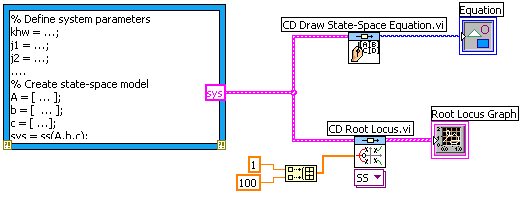
\includegraphics[width=6in]{freqdomain/labview-root-locus.png}
\caption{This VI will plot the root locus along with the poles for
  $K=1$ and $K=100$.  The state space equations for the model will
  also be drawn.}
\label{labview-root-locus}
\end{figure}

LabVIEW also provides an interactive root locus plotter.  You vary the
gain and directly see how the poles of the system move.  Invoke the
interactive root locus plotter using the command \texttt{rlocfind(SYS)}
in a MathScript node where SYS is the name of your model. Things you
might want to know:

\begin{enumerate}
\item You might have to change the feedback type to positive depending
  on how you juggled the signs around in your model.  

\item When you close the interactive root locus, the \texttt{rlocfind}
  function returns the selected gain.  You can output the gain and use
  it in your simulation to test it.  See
  Fig. \ref{mathscript-rlocfind}.
\end{enumerate}

\begin{figure}[h!]
\centering
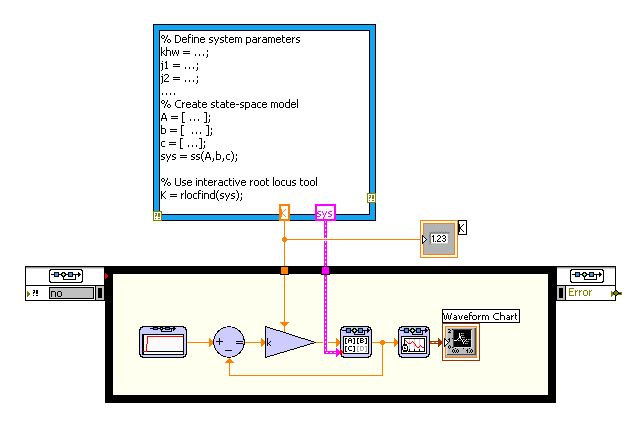
\includegraphics[width=6in]{freqdomain/mathscript-rlocfind.png}
\caption{This VI uses the interactive root locus plot to choose a gain
  and simulates the step response for that gain.}
\label{mathscript-rlocfind}
\end{figure}

\ejnote{I'm recommending the MathScript interactive version.  I know
  the one you refer to wasn't installed with the disks we let them
  take home, and so it might not be on the lab computers.}


\subsection{Bode \label{sec-bode}}
\subsection{Nyquist \label{sec-nyquist}}


%\begin{figure}[h!]
%\centering
%\includegraphics[width=6in]{template/graphic}
%\caption{A LabVIEW-related graphic}
%\label{fig-LabVIEWgraphic}
%\end{figure}

%\begin{wrapfigure}[15]{r}{2in}
%\begin{center}
%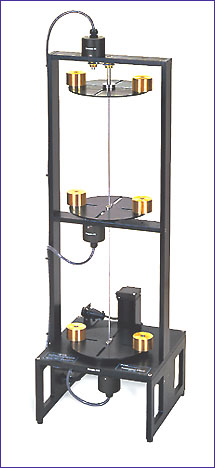
\includegraphics[height=4in]{Lab2/model205}
%\end{center}
%\caption{The ECP Torsional Disk System.}
%\label{fig-ecp}
%\end{wrapfigure}


%% Local Variables:
%% TeX-master: "../LVmanual.tex"
%% End:

